In assembly, computation, and readout of ultracold atoms, laser cooling and trapping techniques play a key role. 
We will give an overview of some techniques, distinguishing the case of a laser close to resonance in \cref{sec:MOT} as well as a laser detuned far away from atomic resonance in \cref{sec:ODT}.
Hopefully, it will become clear that the two cases lead to different behavior as well as applications.
\Cref{sec:PracticeRb} discusses laser cooling on a more practical level for Rb, the element that we mainly used on for this work. 
Finally \cref{sec:Sr}, is on the aspects coming into play for Sr specifically, the element we want to use as a qubit.


\section{Magneto-Optical Trap}\label{sec:MOT}

The workhorse for producing clouds of ultracold atoms is the 3D \ac{MOT}. 
In essence, it consists of three sets of counter-propagating beams as well as a magnetic field gradient, together providing a damping as well as a confining force. 
In this way, high density clouds of ultracold atoms can be produced. 

\subsection{Scattering Force}

Consider an atom with ground state $\ket{g}$ and excited state $\ket{e}$ separated by energy splitting $\hbar \omega_0$.
This convention will be used for the remainder of this work.
The energy levels are shown schematically in \cref{fig:2LevelAtom}.
The laser will output at an angular frequency $\omega$ that is near-resonant, but \emph{detuned} slightly from the transition by an amount $\delta$:

\begin{equation}\label{detuning}
	\delta = \omega - \omega_0.
\end{equation}
It will turn out that detuning is one of the most important parameters in laser cooling. 
In this work we will nearly always use $\delta <0$. 
Because of the Doppler effect, the atom 'sees' a slightly higher frequency $\delta'$ when moving towards the light with a velocity $v$: $\delta'=\delta+k v$ and the laser may become resonant, causing the atom to absorb a photon absorbing momentum $\hbar k$ and promoting an electron to the excited state $\ket{e}$.
When spontaneous emission causes the atom to fall back in a time $\tau = 1/\gamma$ where $\gamma$ is the linewidth of the transition, the electron decays back to the ground state, but the emitted photon is emitted in a random direction. 
This can be repeated many times per second at a scattering rate $\Gamma_{\text{sc}}$, described by the Lorentzian \cite{Metcalf1999}

\begin{equation}\label{eq:ScatteringFrequency}
	\Gamma_{\text{sc}} = \frac{ \gamma s_0 /2}{1+s_0+\left[2(\delta+ k v)/\gamma\right]^2},
\end{equation}
where $s_0 = I/I_{\text{\text{sat}}}$ is the saturation parameter as a function of the light intensity $I$ and saturation intensity $I_{\text{sat}}=2\pi^2 \hbar c \gamma/3\lambdaup^3$. Here, $\lambdaup$ is the wavelength of the laser light.
Because the absorption occurs in a fixed direction and the corresponding emission happens in a random direction, the atom will experience a net \textit{scattering} force $F = \hbar k \Gamma_{sc}$.

\subsection{Optical Molasses}

We can reflect the laser beam using a mirror, such that the force works in both directions of the spatial coordinate.
We will only consider one spatial coordinate which we will denote as $z$, but the treatment can be easily extended to 3 dimensions.
The force will not have a contribution for positive velocities $F^+$ as well as for negative $F^-$, making the total force $F^+ + F^-$ from both contributions \cref{eq:ScatteringFrequency} is \cite{Kowalski2010}

\begin{equation}\label{eq:OpticalMolasses}
	F = F^+ + F^- = \frac{\hbar k \gamma s_0}{2}\left\{\
	\left[1 + s_0 + 4\frac{(\delta - kv)^2}{\gamma^2}\right]^{-1}-
	\left[1 + s_0 + 4\frac{(\delta + kv)^2}{\gamma^2}\right]^{-1}
	\right\}.
\end{equation}
We have plotted the result of \cref{eq:OpticalMolasses} in \cref{fig:SpatialDependencePlots} as a function of velocity in units of $\gamma / k$, yielding a result that is dimensionless. Contributions of both beams, as well as their total force, are shown in units of $\hbar k \gamma$.
Doing a series expansion to first order around $v = 0$, it can be shown the force can be linearized as \cite{Metcalf1999}

\begin{equation}\label{eq:ForceLinearized}
	F \sim \hbar k^2 s_0 \frac{8\delta/\gamma}{\left[1+s_0+(2\delta/\gamma)^2\right]^2} v 
	\equiv -\beta v.
\end{equation}
\begin{figure}
\centering
	\begin{subfigure}{.38\textwidth}
		\centering
		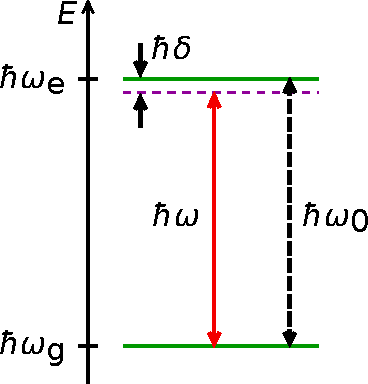
\includegraphics[height=4.5cm]{figures/2LevelAtom.pdf}
		\caption{}
		\label{fig:2LevelAtom}
	\end{subfigure}
	\begin{subfigure}{.61\textwidth}
		\centering
		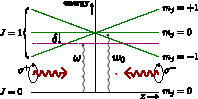
\includegraphics[height=4.5cm]{figures/Molasses.pdf}
		\caption{}
		\label{fig:MOTPlots}
	\end{subfigure}
	\caption{\textbf{a)} Energy level scheme for the 2-level case. 
	The two energies are split by $\mathsf{\omega_e - \omega_g = \omega_0}$.
	The detuning is $\mathsf{\delta = \omega-\omega_0<0}$ is shown as well.
	\textbf{b)} Concept of optical molasses in 1D. 
	Atomic frequency is detuned from the atomic transition by $\mathsf{\delta<0}$.
	Because of the linear magnetic field, for $z>0$, the $\mathsf{\textit{m}_j=-1}$ atoms become resonant with only $\mathsf{\sigma^+}$ light because of selection rules, and vice versa.}
\end{figure}
Where $-\beta$ is the slope of the scattering force around $v=0$. 
For $\delta<0$ the resulting force has a damping effect on the velocity, which if applied in all 3 dimensions can cool atoms to ultracold temperatures. 
Because of the Taylor expansion, \cref{eq:ForceLinearized} is only valid for small velocities $|kv| \ll \gamma$ \cite{Kowalski2010}.

The treatment so far would suggest that this can be used to cool atoms to temperatures of absolute zero. 
This is not the case, as the random character of the scattering force means the atom fluctuates around the equilibrium velocity according to a Brownian motion. 
%balance betweeen cooling and recoil heating. For higher s0 it is doppler broadened by a factor 
For $\delta=-\gamma/2$ and $s_0 =2$, \cref{eq:ForceLinearized} ($\beta$) is at a maximum, yielding the lowest possible temperature achievable using Doppler cooling: the Doppler temperature $T_D$ \cite{Metcalf1999}

\begin{equation}\label{eq:DopplerTemperature}
	T_D = \frac{\hbar}{2k_b} \gamma.
\end{equation}
where $k_b$ is Boltzmann's constant. Apparently, this cooling limit is only dependent on the linewidth of the transition $\gamma$, apart from physical constants. 
For the D$_2$ line of Rb-85 the Doppler temperature is $146$ $\mu$K, whereas for Sr this is about an order of magnitude lower for the red transition.

\subsection{Magneto-Optical Trapping}

Apart from cooling the atoms, we want to trap them at a specific location to increase the density of atoms. 
We can use the Zeeman effect for this, which tells us the atomic energy levels will be split an amount $\Delta E$ according to \cite{Griffiths2004}

\begin{equation}\label{eq:Zeeman}
	\Delta E = \mu_{\emph{B}} g_J m_j B,
\end{equation}
where $\mu_{\emph{B}}$ Bohr magneton, $g_J$ the Landé g-factor, $m_j$ is the magnetic quantum number and $B$ the applied magnetic field. 
The magnetic field is tuned in such a way that it is linear in all 3 dimensions and zero magnitude at the center of the \ac{MOT}.
Because of the Zeeman splitting, the chance of the atom transition being resonant with the laser varies with the position from the origin and the detuning as \cite{Kowalski2010}

\begin{equation}\label{eq:DetuningFull}
	\delta' = \delta + k v + \frac{\mu'B}{\hbar}
\end{equation}
Where $\mu' = (g_e m_e-g_g m_g)\mu_B$ is the effective magnetic moment for the transition \cite{Kowalski2010}. 
To ensure that atoms only absorb momentum kicks opposite to their direction of travel, the laser beams are circularly polarized: $\sigma^+$ from the left and $\sigma^-$ from the right. Because the sign of the Zeeman shift is dependent on the magnetic quantum number $m_j$, selection rules prescribe that atoms displaced by $z>0$ are only resonant with $\sigma^-$-light and vice versa.
This is sketched in \cref{fig:MOTPlots}. Inserting \cref{eq:DetuningFull} in \cref{eq:OpticalMolasses} yields

\begin{equation}\label{eq:MOTfull}
	\frac{F}{\hbar k \gamma s_0} = \frac{1}{2}\left\{\
	\left[1 + s_0 + 4\frac{(\delta - k v - \mu'B / \hbar)^2}{\gamma^2}\right]^{-1}-
	\left[1 + s_0 + 4\frac{(\delta + k v + \mu'B / \hbar)^2}{\gamma^2}\right]^{-1}
	\right\}     
\end{equation}                          
Expanding \cref{eq:MOTfull} around $(v,z) = (0,0)$, keeping only first order terms finally leaves us with \cite{Kowalski2010}

\begin{equation}\label{eq:ForceMOT}
	F_{\text{MOT}}(z,v) \sim -\beta v - \kappa z.
\end{equation}
Where $\beta$ is the same we found in \cref{eq:ForceLinearized} and $\kappa \equiv \mu' \beta /\hbar k \cdot \partial B/\partial z$. 
Apart from the dampening force, we now also have a restoring force. 
When applied in 3 dimensions this can be used to make clouds of ultracold atoms. The behavior of \cref{eq:ForceMOT} is shown in \cref{fig:SpatialDependencePlots}.

\begin{figure}
    \centering
    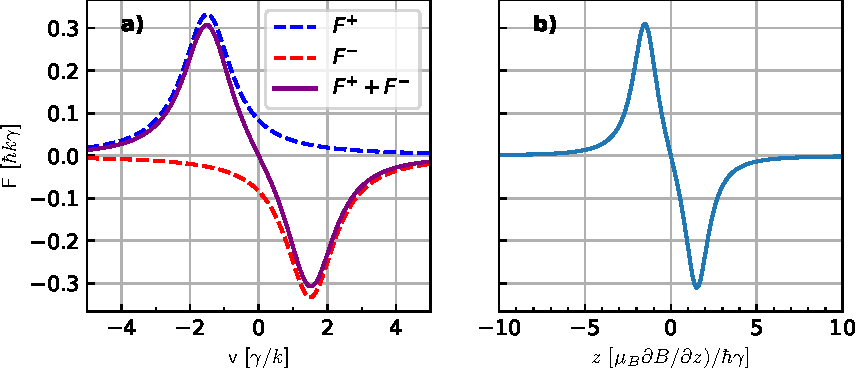
\includegraphics[width=0.9\linewidth]{figures/SpatialVelocityDependence.pdf}
    \caption{\textbf{a)} Optical molasses: contributions from the lasers in both directions $\mathsf{\textit{F}^+}$ and $\mathsf{\textit{F}^-}$ are shown, as well as the total force. Spatial force of the MOT beams and magnetic field gradient. Forces are dimensionless by dividing by $\mathsf{\hbar \textit{k} \gamma}$.}
    \label{fig:SpatialDependencePlots}
\end{figure}

\section{Optical Dipole Traps}\label{sec:ODT}

After atoms are cooled to ultracold temperatures in a \ac{MOT}, they are typically loaded in another type of trap: the \ac{ODT}. 
An ODT uses far-off-resonant light. Though this means that the coupling and therefore the trapping is weaker, it has negligible scattering, which is important to maintain coherence of quantum states. 

\subsection{Working Principle}

We consider a radiation field with complex electric field vector $\mathbf{E}$. 
This field will induce a dipole moment $\mathbf{p}$ in the atom according to 
	
\begin{equation}\label{eq:DipoleMoment}
	\mathbf{p} = \alpha \mathbf{E}.
\end{equation}
Herein $\mathbf{p}$, $\alpha$ and $\mathbf{E}$ are all defined as complex variables. Consequently, the dipole potential will interact with the electric field leading to and an interaction dipole potential $U_{\text{dip}}$ as a function of the position vector $\mathbf{r}$ \cite{Grimm2000}:

\begin{equation}\label{eq:DipolePotential}
	U_{\text{dip}}(\mathbf{r}) = 
	-\frac{1}{2} \left\langle \mathbf{p}\cdot\mathbf{E} \right\rangle=
	- \frac{\operatorname{Re}(\alpha)}{2\epsilon_0 c} I(\mathbf{r}),
\end{equation}
where the $\left\langle\right\rangle$ brackets denote the time average.
We average over this rapidly varying phase term, yielding a factor $1/2$ \cite{Grimm2000}.
Furthermore we used $I(\mathbf{r}) = \epsilon_0 c |\mathbf{E}(\mathbf{r})|^2/2$ where $\epsilon_0$ is the electric constant. 
The dipole force thus scales with the part of the polarizability that is in phase with the light field.
The gradient of \cref{eq:DipolePotential} gives rise to the dipole force:

\begin{equation}\label{eq:DipoleForce}
	\mathbf{F}_{\text{dip}}(\mathbf{r}) = - \frac{\operatorname{Re}(\alpha)}{2\epsilon_0c}\nabla I(\mathbf{r})
\end{equation}
The dipole force can be used to coherently trap our qubits. 
To maximize the dipole force \cref{eq:DipoleForce}, 
we have to maximize the gradient of the light intensity profile.
This can be done by focusing the laser to the smallest possible spot.
How this can be done is explained in \cref{ch:tweezer}. 
Another quantity of interest is the scattering rate.
The scattering rate from the ODT can be found by averaging over the product of the temporal derivative of the dipole moment with the electric field \cite{Grimm2000}

\begin{equation}\label{eq:ScatteringRate}
	\Gamma_{\text{sc}}(\mathbf{r}) = \frac{\left\langle \mathbf{p} \mathbf{E} \right\rangle}{\hbar \omega}
	 = \frac{\operatorname{Im}(\alpha)}{\hbar \epsilon_0 c} I(\mathbf{r}).
\end{equation}
\Cref{eq:DipoleForce,eq:ScatteringRate} are expressions that are valid for arbitrary light fields $I(\mathbf{r})$ and polarizabilities $\alpha$.
In \cite{Grimm2000}, a classical expression for $\alpha(\omega)$ was derived, from which it can be deduced that the relation between the trap depth and scattering rate is

\begin{equation}\label{eq:RelationUG}
    \hbar \Gamma_{sc} =\frac{\gamma}{\Delta} U_{\text{dip}},
\end{equation}
where $\Delta$ is the detuning in the far-off-resonant regime. 
Thus, by increasing $\Delta$, the scattering rate decreases more rapidly than the trap depth. 
This is a key element in optical dipole traps. 
In the next section, we will derive a useful expression for the dipole potential of parameters that can be controlled using experimental parameters using a semi-classical description.

\subsection{Semi-Classical Description}

In the semi-classical treatment, a quantized energy level is considered, along with a classical light field. 
We can write down a general expression for the the light field propagating in the $z$-direction polarized in the $\bm{\hat{\epsilon}}$ direction perpendicular to it:
\begin{equation}\label{eq:ClassicalField}
	\mathbf{E}(z,t) = \mathbf{E}_0 \cos{(k z - \omega t)} 	\bm{\hat{\epsilon}}
\end{equation}
As a starting point, we will consider an atom with two eigenstates: $\ket{g}$ (ground) with energy $\hbar \omega_g$ and $\ket{e}$ (excited) with $\hbar \omega_e$, see \cref{fig:2LevelAtom}. 
Then the atomic Hamiltonian in this basis reduces to \cite{Loudon2000}


\begin{equation}\label{eq:AtomHamiltonianMain}
	\mathcal{H}_A = \hbar \omega_g \ket{g}\bra{g} + \hbar \omega_e \ket{e}\bra{e}
\end{equation}
The radiation field is modeled as a time-dependent perturbation, leading to the Hamiltonian \cite{Leeuwen2017}

\begin{equation}\label{eq:PerturbationMain}
	\mathcal{H} = \mathcal{H}_A + \mathcal{H}_{I}(t),
\end{equation}
We can write down the combined wave function in the basis of the unperturbed eigenstates, its time evolution given by

\begin{equation}\label{eq:TwoLevelMain}
	\ket{\psi(t)} = c_g(t) e^{-i \omega_g t} \ket{g} + c_e(t) e^{-i \omega_e t} \ket{e}.
\end{equation}
In appendix \ref{ch:LightMatter} the Schrodinger equation is solved for the 2-level atom using the dipole approximation as well as the \acf*{RWA}. 
This leads to the following matrix equation for the situation of a 2-level atom of \cref{fig:2LevelAtom} \cite{Foot2005}

\begin{equation}\label{eq:MatrixEvolution}
	i \hbar \begin{pmatrix}
		\dot{c}_g \\ 
		\dot{c}e
	\end{pmatrix}
	= \frac{\hbar}{2} \begin{pmatrix}
		\delta & \Omega \\ \Omega^* & -\delta 
	\end{pmatrix} 
	\begin{pmatrix}
		c_g \\ c_e
	\end{pmatrix},
\end{equation}
where the coupling between the atomic eigenstates and the radiation field is described by the Rabi frequency, which is for this two-level system defined as \cite{Metcalf1999}:

\begin{equation}\label{eq:RabiFrequencyMain}
	\Omega \equiv \frac{e E_0}{\hbar} \bra{g}\mathbf{r}\ket{e}.
\end{equation}
The Hamiltonian of \cref{eq:MatrixEvolution} has eigenvalues 

\begin{equation}\label{eq:EigenValues}
	E_{\pm} = \pm
	\frac{\hbar}{2} \sqrt{\Omega^2+\delta^2}.
\end{equation}
Assuming $|\delta| \gg \Omega$, the eigenenergies are thus 

\begin{equation}\label{eq:SemiClassicalEigenvalues}
	E_g \sim  \frac{\hbar \delta}{2} +\frac{\hbar \Omega^2}{4 \delta}, \quad
	E_e \sim -\frac{\hbar \delta}{2} -\frac{\hbar \Omega^2}{4 \delta}.
\end{equation}
When turning on the laser, the energies are thus shifted by an amount $\Delta E = E(\Omega)-E(\Omega=0)$. 
This is called the light shift or AC Stark shift \cite{Metcalf1999}, sketched in \cref{fig:DipoleForce}.

\begin{figure}
    \centering
	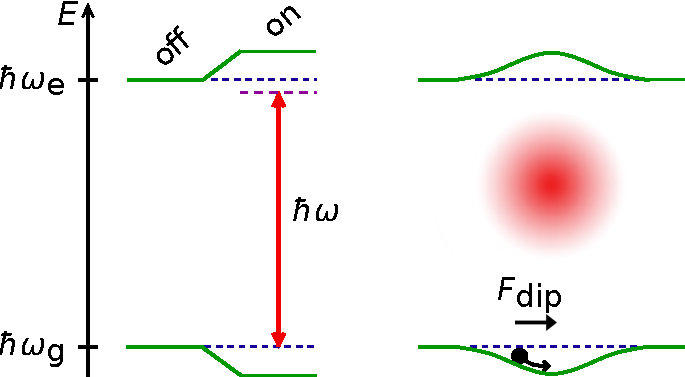
\includegraphics[height=3.8cm]{figures/LightShift.pdf}
	\caption{Light shift for a two-level atom when the off-resonant laser is turned on, as well as the spatially varying light shift for a laser beam profile for $\mathsf{\delta<0}$. 
	The gradient of this potential gives rise to the dipole force denoted in the figure as $\mathsf{\textit{F}_{\text{dip}}}$.}
	\label{fig:DipoleForce}
\end{figure}

\begin{equation}\label{eq:Stark}
	\Delta E_{e,g} \sim \pm \frac{\hbar \Omega^2}{4 \delta}.
\end{equation}
\Cref{eq:Stark} is the main take-away from this section.
The light shift is proportional to the light intensity over the detuning: $\Omega^2 / \delta \propto I / \delta$.
Because scattering is kept to a minimum, atoms in practice only occupy the ground state.
For $\delta <0$ ('red detuned'), the ground state light state is negative. 
So for a spatially varying detuning, the light shift will also vary locally.
This behavior of \cref{eq:Stark} is shown in \cref{fig:DipoleForce}. 


\section{Laser Cooling in Practice}\label{sec:PracticeRb}

In the experimental section of this work we used \ac{Rb} because we had the diode lasers available that are needed for this element.
Also, Rb has a high vapor pressure, simplifying the process of loading the \ac{MOT}.
We review some core features of this element, limiting ourselves to the properties of interest for laser cooling and trapping applications.
For more background on Rb, the interested reader is referred to \cite{Steck2008}.


\subsection{Rubidium}

Rb only has one valence electron, which has ground state denoted by quantum numbers $L=0, S=1/2$ leading to $J=1/2$, meaning this state can be labeled in the standard notation as $5^2S_{1/2}$.
The closest excited state is the $L=1$ (D-line), which is split in fine splitting levels $J=1/2$ ($5^2P_{1/2}$, D$_1$ line) or $J=3/2$ ($5^2P_{3/2}$, D$_2$ line).
The splitting is quite substantial: the D$_2$ line has a wavelength of $\sim780$ nm whereas for D$_1$ this is $\sim$ 795 nm.

But apart from the fine splitting, there is also a hyperfine splitting, which is specifically of interest for laser cooling.
For Rb-85, the nuclear spin $\mathbf{I}=5/2$, which will couple with $\mathbf{J}$, leading to a total atomic angular momentum $\mathbf{F} = \mathbf{J} + \mathbf{I}$.
Now, $F$ can take for the ground state values $F=2,3$ and for the excited state $F=1,2,3,4$ \cite{Steck2008}. 
Because of selection rules, the transitions have to satisfy $\Delta F = -1, 0, +1$. 
This means that the $F = 3 \rightarrow F'=4$ is a special transition: it is \textit{closed}, meaning once excited to $F'=4$ by some cooling laser, selection rules forbid the atom from decaying back to anything else than $F=3$. 
This cycle can be repeated millions of times per second, leading to efficient cooling.

While the laser is tuned very closely to the $F = 3 \rightarrow F'=4$ trapping/cooling transition, from \cref{eq:ScatteringFrequency} it can be deduced that even further away from this resonance, in the tails of the Lorentzian, there is still a slim probability that the $F=3 \rightarrow F'=3$ will occur.
Consequently, these atoms can decay to $F=2$, leaving the closed loop.
While the off-resonant excitation change might be small, when cycling millions of times per second it will be detrimental. 
To combat this, a Rb \ac{MOT} needs another \textit{repump} laser, that re-introduces the lost atoms in the cycle via the $F'=3$ transition.
The hyper-fine splitting of Rb for the ground and excited state, as well as the lasers needed are shown in \cref{fig:D2line}.
In \cref{ch:implementation} we elaborate more on how the MOT was realized experimentally. 

\begin{figure}
    \centering
    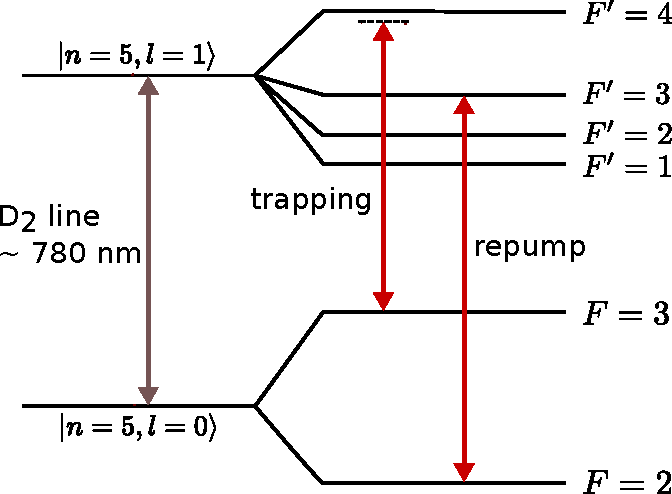
\includegraphics[width=0.48\linewidth]{figures/D2line.pdf}
    \caption{(Hyper)-fine level structure of the Rb-85 $\mathsf{5^{2}S_{1/2} \rightarrow 5 ^2P_{3/2}}$ (D$\mathsf{_2}$) line. Also shown: cooling/trapping transition as well as repump. Figure not to scale}
    \label{fig:D2line}
\end{figure}


\subsection{Magnetic Field}

As is clear from \cref{fig:SpatialDependencePlots}, a magnetic field gradient is needed.
To produce this gradient in 3 dimensions, typically an Anti-Holmholtz configuration is used. 
This consists of two concentric coils with radius $R$, spaced a distance $R$ from each other. 
The current that is run in the coils is opposite in direction, such that the magnetic fields cancel but the magnetic fields in the center point between the coils is not.
Typically, a magnetic field gradient of $\partial B/\partial z \sim 10-15$ Gauss is used.
Because of $\nabla \cdot \mathbf{B}=0$, the field in the $x$ and $y$ directions is a factor 2 weaker. The experimental details are elaborated upon in \cref{ch:implementation}.

\subsection{Optical Trap Depth}

In reality, Rb is not two-level systems, but inhibits a more more complex level structure, e.g. hyperfine splitting.
Because we are only interested in the ground state Stark shift, we will limit ourselves to excited states $\ket{e_j}$ coupled to the ground state $\ket{g}$, such that the ground state dipole potential is a sum of contributions from \cref{eq:Stark}:

\begin{equation}\label{eq:MultiStark}
    \Delta E_{g} = \frac{\hbar}{4} \sum_j \frac{\Omega_{g,e_j}^2}{\Delta_{g,e_j}},
\end{equation}
where $\Delta_{g,e_j}$ are the detunings and $\Omega_{g,e_j}$ the Rabi frequencies of the transition $\ket{g} \rightarrow \ket{e_j}$ \cite{Brossard2020}. 
In general, transitions to all (hyperfine) energy levels have to be taken into account. 
However, for linearly polarized light, all hyperfine energy levels turn out to have the same coupling, thus we can omit the sum over the hyperfine levels. Using the $J \rightarrow J'$ dipole matrix elements for linearly polarized light \cite{Steck2008}:

\begin{equation}
    |\bra{J} | e \mathbf{r} | \ket{J'}|^2 = \frac{3 \pi \epsilon_0 \hbar c^3}{\omega_{0,j}^3} \frac{2J'+1}{2J+1} \gamma,
\end{equation}
and only taking into account the $J=1/2 \rightarrow J'=1/2$ (D$_1$) and $J=1/2 \rightarrow J'=3/2$ (D$_2$ lines), \cref{eq:MultiStark} reduces to

\begin{equation}\label{eq:RbTrapDepth}
    U_{\text{dip}} = \frac{3\pi c^2}{2} \left(
    \frac{1}{3}\frac{\gamma_1}{\Delta_1 \omega_{0,1}^3} + \frac{2}{3}\frac{ \gamma_2}{\Delta_2 \omega_{0,2}^3} 
    \right) I,
\end{equation}
where the subscripts 1 and 2 denote the contributions from the D$_1$ and D$_2$ lines. 
To effectively load atoms from the MOT in the bottom of the tweezer, the tweezer trap depth $U_0$ should be larger than the temperature of the atoms. 
The temperature was measured by Rik van Herk \cite{Herk2022} and is roughly 200 $\mu$K.
Therefore, we used a trap depth of $U_{\text{dip}} /k_b \sim 1.5$ mK for the tweezer, here $k_b$ denotes Boltzmann's constant, or $U_{\text{dip}} / h \sim 30$ MHz.
Using \cref{eq:RbTrapDepth} and the relation between light intensity and power $P$ of a Gaussian beam $I = 2P/\pi w^2$, we find we can estimate the amount of power needed given the wavelength and waist of the laser beam. 

Needing a far-off-resonant wavelength, for Rb a range of $795 - 850$ nm can be used.
The lower end of this spectrum gives deeper traps from \cref{eq:Stark} for the same laser power, but it will also be harder to separate atomic fluorescence at $\sim 780$ nm, because in practice dichroic filters used for this are imperfect.
We settled at a compromise of $820$ nm for the wavelength of this Rb optical tweezer, which is very close to the wavelength used for Sr as well (see \cref{sec:Sr}). As for the waist, as typical waist for this wavelength is $\sim 0.8$ $\mu$m, as more thoroughly described in \cref{ch:tweezer}. Plugging all of this in \cref{eq:RbTrapDepth} we find we need about $1.8$ mW of laser power, which is specific for this trap depth, wavelength and waist.


\section{Laser Cooling: Strontium}\label{sec:Sr}

Contrary to the one valence electron in \ac{Rb}, \ac{Sr} is a alkali-earth (group 2) element, meaning it has two valence electrons.
This means the level structure is more complicated, but this also opens up many new and interesting possibilities unavailable to group 1 elements.
Some of the properties of Sr make it an excellent candidate for applications in quantum computing.
For a far more extensive coverage of Sr, the reader is referred to \cite{Stellmer2013}. 
Here, we will review some basic properties of Sr relevant for laser cooling it to ultracold temperatures and using it as a qubit.

To start off, Sr has 4 stable isotopes.
Three of them are bosonic, with ${}^{88}$Sr being the most abundant at $\sim82.6\%$. There is one stable fermionic isotope: ${}^{87}$Sr has a nuclear spin of $I=9/2$ and an abundance of $\sim7.0\%$ \cite{Coursey1999}.
Initially, we plan to run the machine in Eindhoven on \textsuperscript{88}Sr. 
Because of the lack of hyper-fine structure, this isotope is a bit easier to work with.
Though, in principle, one can use all isotopes in the same machine as the energy splitting between the isotopes is in the hundreds of MHz regime, easily covered by AODs and EOMs \cite{Stellmer2013}.

\subsection{Relevant Transitions}

A simplified version of the level diagram of \textsuperscript{88}Sr is shown in \cref{fig:SrLevel}. 
The notation is $(n_1l_1 n_2l_2)^{2S+1}L_J$ where $n_{1,2}$ is the principal and $l_{1,2} = s, p, d, \ldots$ the azimuthal quantum number. 
Furthermore $S$, $L$ and $J$ are the total spin, orbital angular momentum, and total angular momentum quantum numbers respectively \cite{Cowan1981}. 
This level scheme shows 6 out of 7 lasers to be used in this experiment. 

\begin{itemize}
	\item 461 nm. Broad transition, meaning a strong scattering force (\cref{eq:ScatteringFrequency} and high absorption-emission cycling frequency.
	This is useful to slow down the hot atomic beam coming from the oven, as well as catching the atoms in a so-called blue \ac{MOT} with 'hot' temperatures of $\sim$ 1 mK.
	
	\item 689 nm. Because it is much narrower than the blue transition, its Doppler temperature \cref{eq:DopplerTemperature} is much lower at $179$ nK, although in practice cooling is limited by the recoil limit to some $\sim 1$ $\mu$K \cite{Stellmer2013,Boyd2007}.
	
	\item 698 nm. The ultra-narrow clock transition ($\gamma = 1$ mHz). 
	Used in atomic clocks because of its spectroscopic accuracy \cite{Bloom2014}.
	It will turn out that this feature can be put to good use in quantum computers as well, and we will use it to coherently 'drive' the qubits between the qubit basis states using this clock transition. 
	More about this in \cref{sec:QubitScheme}.
	
	\item 679, 688, and 707 nm. 
	All repump lasers. 707 and 688 are used to cycle back atoms from ending up in ${}^3P_2$ from the decay channel shown by the grey dotted line in \cref{fig:SrLevel}. The 679 nm laser is used to prevent repump leaks to ${}^3P_0$ \cite{Stellmer2013,Xu2003}.
\end{itemize}

There will also be a 813 nm laser used for producing the optical dipole trap potentials.
This is also the most powerful laser, as it determines the limit of qubits (optical tweezers) one can make. 
One can find more about this laser in \cref{sec:Magic}.

\begin{figure}
	\centering
	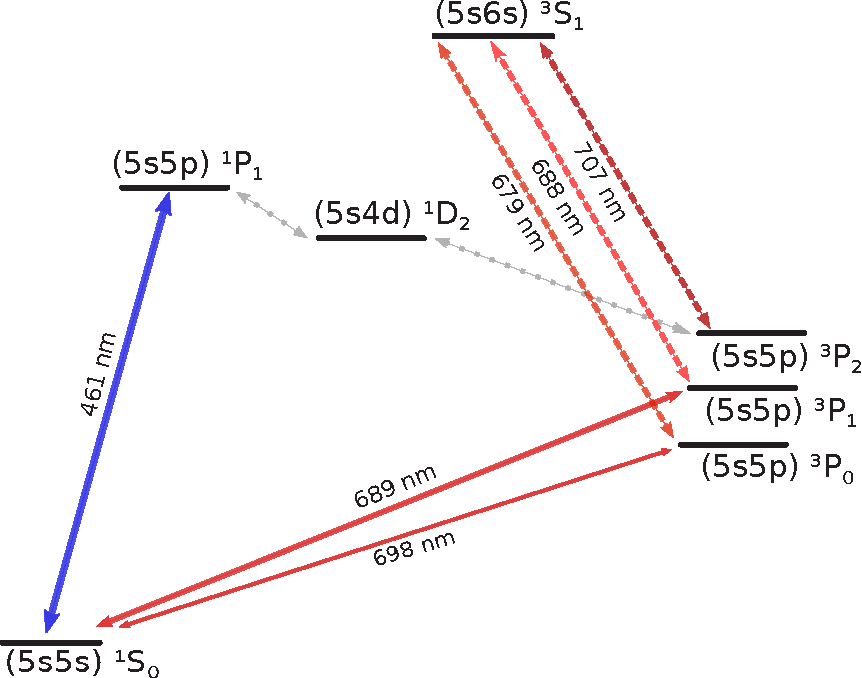
\includegraphics[width=0.55\linewidth]{figures/SrLevel.pdf}
	\caption{Simplified level scheme for \textsuperscript{88}Sr. 
	Shown: blue transition for initial slowing and cooling.
	Narrower 689 nm transition of the red \ac{MOT}, and the \textsuperscript{1}S\textsubscript{0} - \textsuperscript{3}P\textsubscript{0} clock transition, which we will be used to drive the qubits. 
	To increase density and trap lifetime 3 repump lasers are used. 
	Not shown: 813 nm dipole trapping laser because it is driven far-off-resonant from atomic transitions. Energies not to scale. Figure made by Ivo Knottnerus.}
	\label{fig:SrLevel}
\end{figure}

\subsection{Laser Cooling and Trapping of Sr}

Because the melting temperature of Sr is $777$ ${}^{\circ}$C, it requires a bit more work to load Sr atoms in a magneto-optical trap.
To get any relevant vapor pressure, the Sr is heated in an oven after which it sublimates. 
To obtain a small atomic beam divergence, the atoms are directed through a bundle of high aspect ratio capillary tubes \cite{Stellmer2013}. Because of this heating however, the atoms will be moving too fast to be efficiently captured by the MOT.
Therefore, they are first slowed by a Zeeman slower. 
This machine uses a similar design used in the optical molasses technique, only the slowing beam is only opposing the atomic beam and not traveling along with it. 
A spatially varying magnetic field ensures a wide range of velocities is at some point resonant with the laser according to \cref{eq:DetuningFull}. 

Depending on the length of the Zeeman slower, only a fraction of the atoms will be slowed.
To separate the hot from the cool atoms (the former are unwanted in a vacuum chamber) a deflection stage is used. 
The blue transition of Sr is used for this stage because of the strong scattering force. 
The Zeeman slowing and deflection stage is explained more elaborately in the thesis of Rik van Herk \cite{Herk2022}.

After the deflection stage, the atomic beam enters a glass cell.
In the glass cell, all the magic happens: the magneto optical traps, dipole traps, as well as all the qubit operations (coupling, pulses, readout) happen in this cell.
This is why a glass cell is used: optical access is a valuable asset when using ultracold atoms, where practically all operations consist of using various laser beams.
To allow for longer trap survival times, the glass cell has \ac{UHV} which is separated from the stages preceding it by a differential pumping stage. 

\begin{figure}
	\centering
	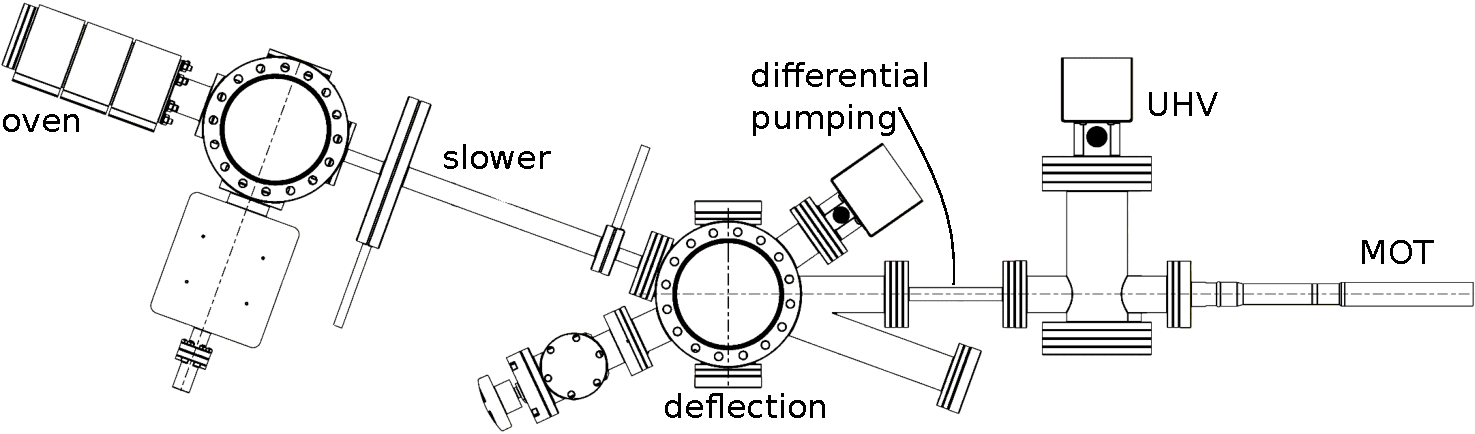
\includegraphics[width=0.8\linewidth]{figures/SrLoading.pdf}
	\caption{Sketch of the vacuum atom source design and vacuum chambers. 
	Starting from the oven, the atomic beam traverses a Zeeman slower, deflection stage, and differential pumping stage before ending in the glass cell (MOT, right). 
	Figure by Patrick de Laat.}
	\label{fig:SrLoading}
\end{figure}

\subsection{Strontium as a Qubit}\label{sec:QubitScheme}

One of the main reasons we want to use strontium atoms for the quantum processing unit is the ${}^3P_0$ state and its very long lifetime. 
The clock transition is forbidden according to selection rules and only opens up after applying a magnetic field for the \textsuperscript{88}Sr isotope \cite{Knottnerus2018}.
Therefore, ${}^3P_0$ is called meta-stable and can be considered a ground state on the time scale of the operation of a quantum processing unit. 
${}^1S_0$ is the other clock state.
Therefore, we effectively have two ground states and we can denote our qubit states as $\ket{g_1}$ and $\ket{g_2}$ (the clock states) as

\begin{equation}\label{eq:QubitManifold}
	\big\{\ket{0},\ket{1}\big\} = 
	\left\{
		\ket{{}^1S_0}, \ket{{}^3P_0} 
	\right\} = 
	\left\{ 
	    \ket{g_1}, \ket{g_2}
	\right\}.
\end{equation}
So we have two long-lifetime states connected by an extremely narrow linewidth coupling between them, that can be used to drive the qubits on the Bloch spheres.
To entangle the qubits, Rydberg dressing can be used \cite{Wu2021} where a small part of a Rydberg state $\ket{r}$ is admixed in the higher energy ground state:

\begin{equation}\label{eq:RydbergDressing}
	\ket{\psi} \sim \ket{g_2} + \epsilon \ket{r}
\end{equation}
The amount of dressing is tuned by the (small) dressing parameter $\epsilon \propto \Omega / 2\delta$ where $\Omega$ is the Rabi frequency of the laser and $\delta$ the usual detuning. 
A Rydberg state is an electronic state with a very high principal quantum number $n$. Rydberg atoms are physically larger, as the electron orbit radius scales $\propto n^2$ \cite{Gallagher1994}. 
As a result of these exaggerated electron orbit sizes, neighboring atoms can 'feel' each other.
For example, the van der Waals interaction coefficient has one of the highest scaling coefficients, scaling as $\propto n^{11}$ \cite{Gallagher1994}. 

Other qubit implementations than the one above are possible as well.
For example, \cite{Barnes2021} uses the fermionic ${}^{87}$Sr and maps the qubit states onto the nuclear spin states $\ket{{}^1S_0, F=9/2, m_F = -9/2}$ and $\ket{{}^1S_0, F=9/2, m_F = -7/2}$.

\subsubsection*{Magic Trapping of Strontium}\label{sec:Magic}

To use the states in \cref{eq:QubitManifold}, they should both be trapped by exactly the same dipole potential to minimize broadening of the transition between them.
Because the trapping potential is wavelength dependent, in general, the trapping potential will not be the same for both qubit states when using the same trapping wavelength, because the polarizability in \cref{eq:DipoleForce}: is wavelength dependent: $\alpha = \alpha(\omega) = \alpha(\lambdaup)$.
Instead, \cite{Katori2003} proposed to use a wavelength where the polarizability $\alpha(\lambdaup)$ is identical for both clock states, causing the differential stark shift $\hbar \times \delta \nu$ to vanish.
Using \cref{eq:DipolePotential}:

\begin{equation}\label{eq:DifferentialStarkShift}
    \hbar \times \delta \nu = U_{\text{dip},1} - U_{\text{dip},0} = 
    \operatorname{Re}\left\{\alpha_1(\lambdaup)-\alpha_0(\lambdaup)\right\} \frac{I}{2 \epsilon_0 c}.
\end{equation}
\begin{figure}
    \centering
    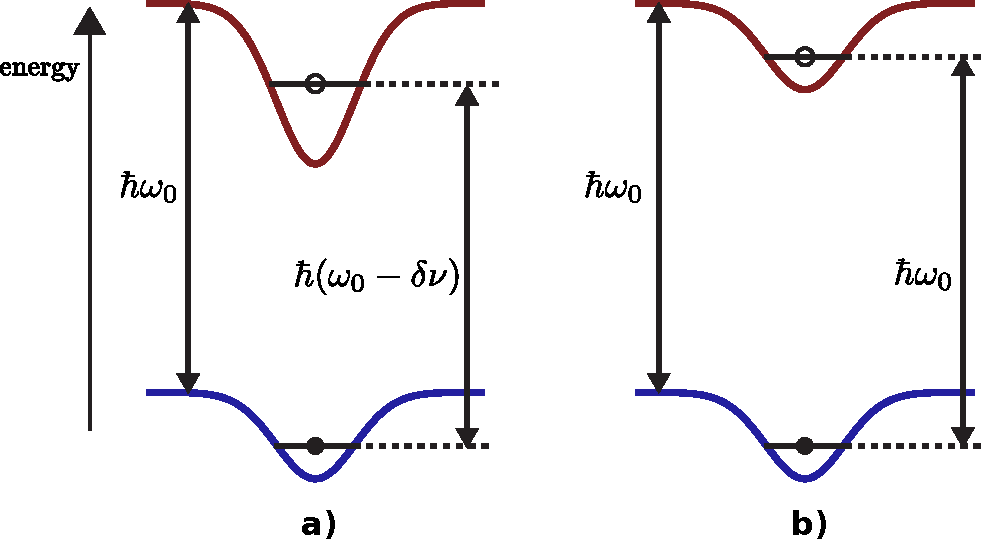
\includegraphics[width=0.65\linewidth]{figures/MagicTrapping.pdf}
    \caption{\textbf{a)} Different trap depths for the ground and excited states lead to spatial variation of the transition frequency called the differential stark shift $\hbar \times \delta \nu$.
    \textbf{b)} Magic trapping: the differential Stark shift is minimized because the polarizabilities of both states is identical.
    Figure adapted from \cite{Lundblad2010}.}
    \label{fig:MagicTrapping}
\end{figure}
The calculation is described in \cite{Madjarov2020,Boyd2007} and was experimentally verified by \cite{Takamoto2005}.
For Sr, the wavelength where the magic condition occurs is roughly 813 nm. 






	

